\section{Experiment II: Novel Speakers}
The first experiment used training and test partitions where a speaker's syllables may appear in both. To more accurately match the potential application, the models in this experiment were tested on novel speakers; an individual's syllables appeared in either the test or train set, but not both. 

Because the number of speakers in the data set is small, at sixty-nine, we opted to evaluate the models using a 10-fold cross validation. Nine of the speakers were randomly set aside as a validation set. We then partitioned the remaining sixty into ten groups of six. A cross validation trial consisted of ten rounds, distinguished by which fold is used as the test set. Meaning, in each round, the models were trained on fifty-four speakers and tested on a set of six novel speakers.

The prior experiment effectively rounded the logistic regression layer's activation to produce the label $Y$. In contrast, the following experiments consider three ways to interpret the activations: syllable, soft-majority, and noisy-OR. The first is simply the un-transformed output from the logistic regression layer $\alpha_{reg}$, when given a single syllable. In contrast, the latter two methods consider all of a speakers' examples. Rather than classifying a syllable, soft-majority and noisy-OR classify a speaker. 

Because the traditional nosiy-OR calculation would be affected by the number of syllables each speaker has, we computed it in log-space and normalized by the number of syllables in the calculation. This allowed us to directly compare the nosy-OR scores between speakers with a varying number of examples.

For the logistic regression activations for all of some speaker's syllables $\{\alpha_{reg}^{(0)}, \alpha_{reg}^{(1)},...,\alpha_{reg}^{(m-1)}\}$ and some integer $k \in [0,m-1]$,

\begin{align}
syllable &= \alpha_{reg}^{(k)},\\
soft-majority &= \frac{1}{m} \sum_{i=0}^{m-1} \alpha_{reg}^{i} \\
noisy-OR &= \frac{1}{m} \sum_{i=0}^{m-1} log(1-\alpha_{reg}^{i})
\end{align}

\ref{fig-exp-2-results} presents the receiver-operator and precision-recall curves for each method of inference while \ref{tab-exp-2-results} lists their respective area under curve (AUC) scores. The soft-majority and noisy-OR methods produced identical results, so the latter's curve is not explicitly shown. 

To gain perspective on these AUC scores, we consider a model which produces a positive classification with probability $\theta$. The majority classifier can be seen as the extreme case, where $\theta = 1$. As $\theta$ increases from $0$ to $1$, the red linear curve in \ref{fig-exp-2-results} is produced. Graphically, we can see that the AUC of this curve is $.5$. 

The models clearly improve upon this baseline for all three methods of inference. Moreover, while all three LSTMs performed similarly in the first experiment, $LSTM-1$ clearly produces the most impressive results on novel speakers. 

As expected, soft-majority and noisy-OR achieved higher scores than syllable level evaluation. It is worth pointing out that these two methods' are more appropriate for practical purposes; we would be remiss to think that an accurate diagnosis could result from a single syllable. 

\begin{table}[h]
\centering
\caption{Experimental results}
\begin{tabular}{|l|c|c|c|}
\hline
\multicolumn{1}{|c|}{}    &   Syllable     &   Soft-Majority         &     Fuzzy-Or         \\ \hline
LSTM-1                      &   .754     &   .854     &     .854       \\ \hline
LSTM-2                      &   .695     &   .785     &     .785       \\ \hline
Bi-LSTM-1                   &   .714     &   .847     &     .847      \\ \hline
\end{tabular}
\label{tab-exp-2-results}
\end{table}


\begin{figure*}[t]
    \centering
    \begin{subfigure}[b]{0.4\textwidth}
        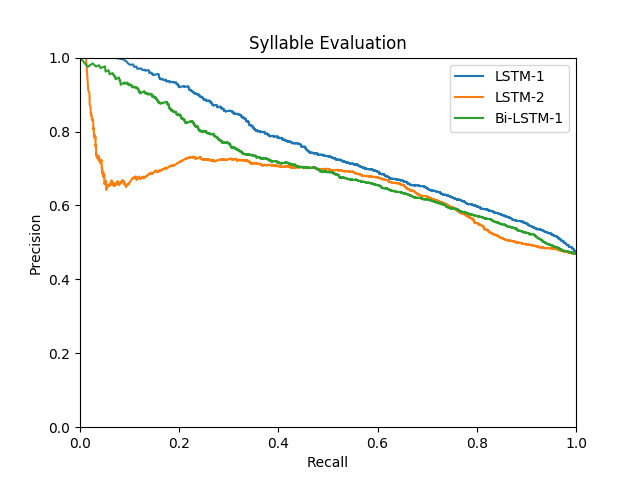
\includegraphics[width=\textwidth]{syl_pr}
        \caption{}
        \label{rfidtest_xaxis}
    \end{subfigure}
    \begin{subfigure}[b]{0.4\textwidth}
        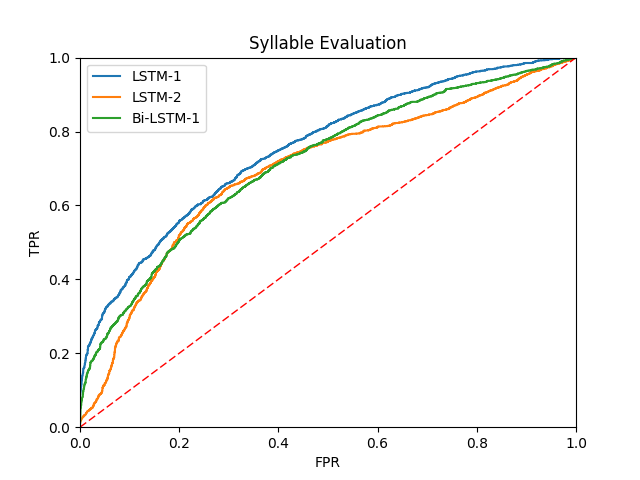
\includegraphics[width=\textwidth]{syl_roc}
        \caption{}
        \label{rfidtest_yaxis}
    \end{subfigure}
    \begin{subfigure}[b]{0.4\textwidth}
        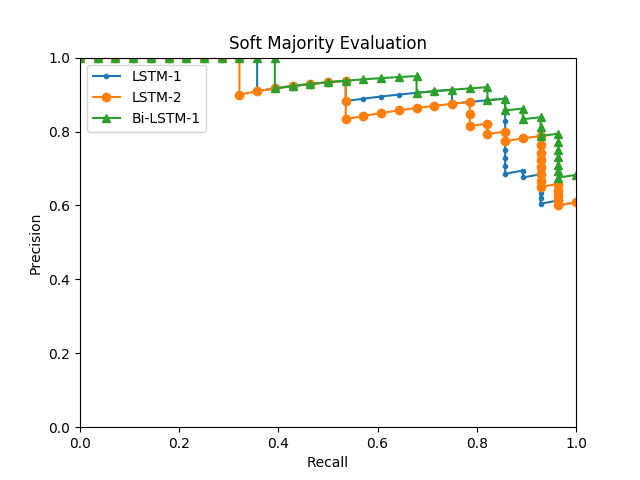
\includegraphics[width=\textwidth]{sm_pr}
        \caption{}
        \label{rfidtest_zaxis}
    \end{subfigure}
    \begin{subfigure}[b]{0.4\textwidth}
        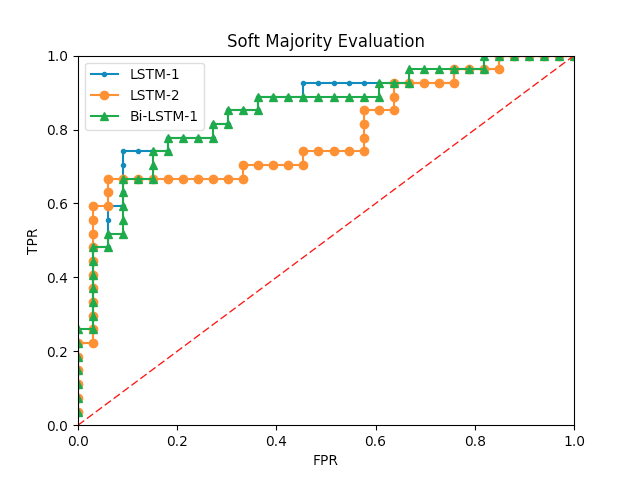
\includegraphics[width=\textwidth]{sm_roc}
        \caption{}
        \label{rfidtest_zaxis}
    \end{subfigure}
    \caption[]{}
    \label{fig-exp-2-results}
\end{figure*}
